%Sample for is295.cls
%Author: Katrina Joy Abriol-Santos
%Reminders: Omit \lipsum commands

\documentclass{is295}
\usepackage{lipsum} %for generating dummy text
\usepackage{hyperref} %for hyperlinks

%\usepackage{showframe} %for debugging the margins
                              
                              
%Replace the values here, various commands depend on this variables  
\renewcommand{\TITLE}{AUTOMATED CATEGORIZATION OF ARTICLES USING NATURAL LANGUAGE PROCESSING}
\renewcommand{\AUTHOR}{MIGUEL V. ABRIOL-SANTOS}
\renewcommand{\DEGREE}{MASTER OF INFORMATION SYSTEMS}
\renewcommand{\ADVISER}{KATRINA JOY M. ABRIOL-SANTOS}
\renewcommand{\FACULTY}{Faculty of Information and Communication Studies}
\renewcommand{\MONTH}{JANUARY}
\renewcommand{\YEAR}{2060}
\renewcommand{\DAY}{01}

% Choose between YES and NO here
\renewcommand{\INVENTION}{YES/NO}
\renewcommand{\PUBLICATION}{YES/NO}
\renewcommand{\CONFIDENTIAL}{YES/NO}
\renewcommand{\FREE}{YES/NO}
% ---------------------

\newcommand{\PROGRAMCHAIR}{DR. RIA MAE H. BORROMEO}
\newcommand{\DEAN}{DR. DIEGO S. MARANAN}

\begin{document}
	
	\begin{frontmatter}
            
		%TITLE PAGE
		\maketitle

            %PERMISSION PAGE
            % This is the University Permission Page. Do not edit the statement here.
% Just put the date

\begin{universitypermission}
    \textbf{University Permission Page} \\\\
    \textbf{\TITLE} \\\\
    I hereby grant the University of the Philippines a non-exclusive, worldwide, royalty-free license to reproduce, publish and publicly distribute copies of this Academic Work in whatever form subject to the provisions of applicable laws, the provisions of the UP IPR policy and any contractual obligations, as well as more specific permission marking on the Title Page.” \\\\
    I specifically allow the University to:
    \begin{enumerate}
        \item Upload a copy of the work in the theses database of the college/school/institute/\\department and in any other databases available on the public internet
        \item Publish the work in the college/school/institute/department journal, both in print and electronic or digital format and online; and
        \item Give open access to the work, thus allowing “fair use” of the work in accordance with the provision of the Intellectual Property Code of the Philippines (Republic Act No. 8293), especially for teaching, scholarly and research purposes.
    \end{enumerate}
    \vspace{0.5in}
    \begin{flushright}
    
    %put the date
    \AUTHOR / Date \\
    Signature over student name and date
    \end{flushright}
\end{universitypermission}

            %APPROVAL PAGE
            \begin{approvalpage}
    \textbf{Approval Page} \\\\
    This paper prepared by \AUTHOR\ with the title: "\TITLE" is hereby accepted by the \FACULTY, U.P. Open University, in partial fulfillment of the requirements for the degree \DEGREE.\\

    \vspace{1in}
    \addsignature{\ADVISER}{Adviser} 
    \vspace{0.5in}
    \addsignature{\PROGRAMCHAIR}{MIS Program Chair}

    \vspace{3in}
    \begin{centering}
    \textbf{\DEAN} \\
    Dean \\
    \FACULTY \\
    \vspace{0.5in}
    Date Signed \\
    \end{centering}
\end{approvalpage}
            
		%ACKOWLEDGEMENT
            % Put you acknowledgement here

\begin{acknowledgement}
    \lipsum[4]
    \lipsum[4]
    \lipsum[4]
    MUST NOT EXCEED ONE PAGE.
\end{acknowledgement}
		
            %ABSTRACT
            % Put your abstract here

\begin{abstractwithpageno}	
    Please use \href{https://writingcenter.gmu.edu/writing-resources/different-genres/writing-an-abstract}{this} as a guide for writing your abstract. \lipsum[4]\ MUST NOT EXCEED ONE PAGE.
\end{abstractwithpageno}
		
		%TABLE OF CONTENTS
		\maketableofcontents
		
		%LIST OF TABLES
		\makelistoftables

		%LIST OF FIGURES
		\makelistoffigures

	\end{frontmatter}
	
	%BODY OF MANUSCRIPT HERE (Use up to 3 levels only, (sec -> subsec -> subsubsec)
	\begin{mainmatter}
		
            %INTRODUCTION
            \section{INTRODUCTION}
    \subsection{Background of the project}
            Your introduction must address the following questions (note that this is a guide, the questions must not be the subsections in the Introduction):
            \begin{itemize}
                \item What is the problem that you are trying to address? 
                \item Why is the problem interesting?
                \item What is the solution of others? Include a summary of what the others are currently doing.
                \item What is the background of the proposed solution?
                \item What is being proposed in this document? Include the following: summary of methodology and the expected results
            \end{itemize}
        \lipsum[4]
    \subsection{Objectives}
        What do you wish to achieve in your capstone project? Write one general and at least three specific objectives of your project. The objectives must:
            \begin{itemize}
                \item be clear, concise, declarative statement;
                \item provide direction to investigate the variables in the study;  
                \item focus on ways to measure the variables, to identify or describe them;
                \item identify relationships between variables;
                \item indicate results sought by the project proponent at the end of the process;
                \item be closely related to the statement of the problem; and
                \item be SMART: Specific, Measurable, Attainable, Realistic, Time-bound.
            \end{itemize}
    \subsection{Scope and Limitations}
        In a research or capstone project, the scope and limitations are essential elements that guide the work to stay focused and define the extent of the content to be covered. 
        \subsubsection{Scope}
            The scope of a study refers to the extent or boundary of the research and defines where the project will be deep-diving. It outlines what the project will encompass and also determines its size and the parameters to work within, including specific objectives, activities, resources, methodologies, and deliverables. For instance, if the project is about developing an AI model to predict stock prices, then the scope could include analyzing given datasets, pattern recognition, implementing machine learning algorithms, testing the model's accuracy, and more.\\
            In terms of scope, a clear definition is a vital step to avoid research deviations. It ensures that the project remains on track without straying into unrelated areas. If the scope is not well defined, the study can easily grow beyond your control.
        \subsubsection{Limitations}
            The limitations of a study are potential weaknesses or problems encountered during the study due to constraints on methodology or resources. These might include a lack of available or reliable data, time or financial constraints, lack of access to technology or software, and the assumptions you've had to make due to such constraints. \\
            For example, in the above-mentioned AI model, a limitation could be the unavailability of real-time stock data for accurate testing, or perhaps certain algorithms couldn't be used due to software limitations.

            %REVIEW OF EXISTING ALTERNATIVES
		\section{REVIEW OF EXISTING ALTERNATIVES}
This chapter examines the diverse approaches employed by animal welfare organizations to facilitate animal adoption and sponsorship, focusing on both local and international models. 


\textbf{Pet Adoption Initiatives:}

\begin{itemize}
 \item \textit{The Philippine Animal Welfare Society (PAWS)} which maintains web pages dedicated to showcasing the stories of rescued animals residing in their sanctuary that have been rehabilitated and are now healthy enough for adoption (https://paws.org.ph/adopt/). Visitors can submit their adoption applications along with preliminary responses to help provide initial assessment whether they would be a suitable match for the animal. The assessment process and subsequent steps, such as in-person meet-ups, are conducted manually.

  \item \textit{The Compassion and Responsibility for Animals (CARA Welfare Society)} offers additional opportunities for public involvement. Their website features information on various animals available for adoption, fostering, and/or donation. To facilitate the process, CARA provides Google Forms to capture application details. Subsequent steps, similar to those of PAWS, are handled manually.

  \item \textit{Petfinder.com, powered by the Petfinder Foundation}, is a U.S.-based platform dedicated to preventing animal euthanasia by supporting shelters and rescue organizations. Through grants and resources, Petfinder enhances adoption rates and promotes responsible pet ownership. The platform makes pet adoption more accessible by providing a comprehensive list of adoptable pets in users' local areas, streamlining the process through its user-friendly web application. By connecting potential adopters with animals in need of a home, Petfinder helps reduce the number of pets in shelters and ensures more animals find their forever families.
 \end{itemize}


\textbf{Design Related Platforms:}

\begin{itemize}
 \item \textit{Adoption Date }is an interactive mobile platform developed by the Society for the Prevention of Cruelty to Animals (SPCA) to support small shelters in Hong Kong. This platform enables users to explore detailed animal profiles and express their interest in adopting or fostering animals in need. Users can stay updated with push notifications about animals available for fostering or adoption, ensuring they never miss an opportunity to help. With a focus on engagement and real-time updates, Adoption Date streamlines the adoption process and connects potential adopters and foster caregivers with animals awaiting their forever homes.
 \end{itemize}

                


		%PROJECT DETAILS
            % Put the project details here

\section{PROJECT DETAILS}
    \lipsum[6]
    %FIGURE INSERTION SAMPLE
    \begin{figure}[ht]
    \begin{center}
        \vspace{4ex}
        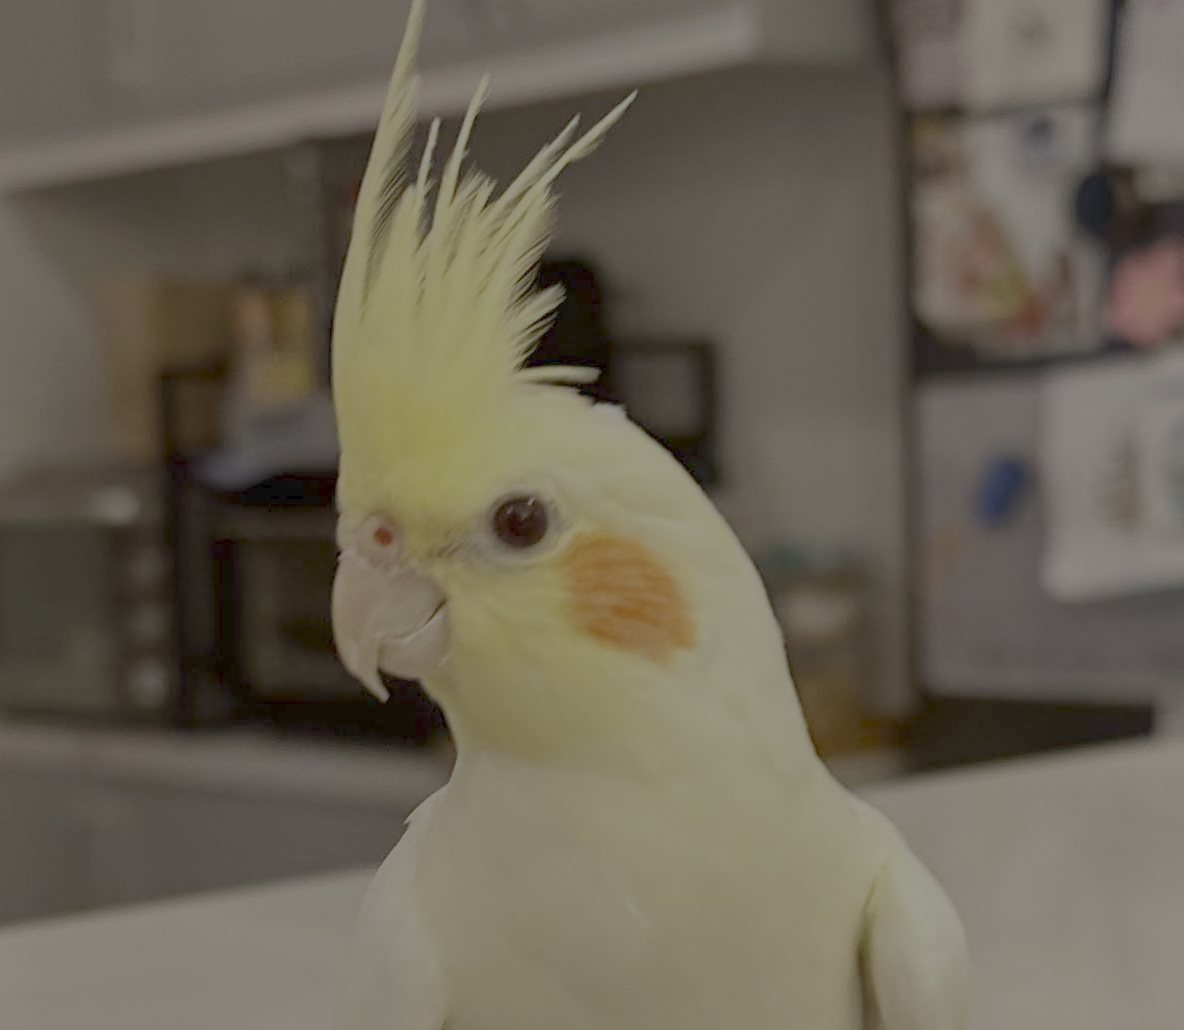
\includegraphics[width=200px]{Texfiles/images/ranger.png}
        \label{fig:Test Caption Figure}	
        \caption{Test Caption Figure}
    \end{center}
    \end{figure}
    \lipsum[4]
        \subsection{Overview}
        This is a brief description of the proposed system.
        \subsection{Project Framework}
        A project framework in is the overarching structure or outline that guides the planning, execution, and management of the project. 
        \subsection{Materials/Technologies Used}
        This includes the technologies to be used or used in the development of the system and their descriptions, and how they are utilized in the project.
        \subsection{System Design}
        Include functional and non-functional requirements and their descriptions, user case design, database design, etc. 
        \subsection{Implementation}
        The details of the implementation of the system. For IS 295A, you need to include an implementation plan and include a Gantt chart as one of the appendices. For IS 295B, include screenshots of the system and their descriptions.


            %PROJECT ASSESSMENT
            % Put the project assessment here

\section{Project Assessment}
    \subsection{User Testing}
    \begin{itemize}
        \item How did you test the system?
        \item How did you find bugs? 
        \item Give all the details: the test specifications, the number of users who tested it, etc.
        \item Explain results. How did you fix the bugs? 
        \item Did you do regression testing after fixing the bugs?
    \end{itemize}
    \subsection{Security Testing}
        Use \href{https://www.zaproxy.org/ }{this} tool for testing the security of your system. What are the security vulnerabilities of your system? How did you/will you address that?

            %RESULTS AND DISCUSSION
            % Put the results and discussion here

\section{RESULTS AND DISCUSSION}
    What are the things you learned as you did this project? What are the challenges that you encountered? Share relevant insights. 
    \lipsum[4]

    %TABLE INSERTION SAMPLE
    \begin{table}[ht]
    \vspace{4ex}
    \centering
        \caption{Test Caption Table}   
        \label{table:Test Caption Table}
        \begin{tabular}{llllll}
        \hline
        \hline
        1 & 2 & 3 & 4 & 5 & 6 \\ \hline
        1 & 2 & 3 & 4 & 5 & 6 \\
        1 & 2 & 3 & 4 & 5 & 6 \\
        1 & 2 & 3 & 4 & 5 & 6 \\ \hline\hline
        \end{tabular} 
    \vspace{4ex}
    \end{table}
    
    \lipsum[8-10]
    \lipsum[5]
		
		%SUMMARY AND CONCLUSION
            % Put the summary and conclusion here

\section{SUMMARY AND CONCLUSION}
    Here's a \href{https://essay-lib.com/write-conclusion-research-paper/}{guide} on how to write your conclusion.
    \lipsum[4]

            %FUTURE WORK
            % Put the future works here

\section{FUTURE WORK}
    This section of the document points towards potential improvements, expansions, or new lines of inquiry that follow from your project. This section is crucial – not just for academic projects, but also for industry projects – as it acknowledges that research is an ongoing process and that one project can't cover every aspect of the topic.\\
    \lipsum[4]
            
		%REFERENCES
		%Parameter is the references bib file without extension
		\makereferences{references}
			
	\end{mainmatter}
\end{document}
